\section{Methods}
\label{sec:methods}

\subsection{Software Tools and Libraries}
\label{subsec:libs}

//TODO

\subsection{Development Data Preparation}

In the following, the data preparation techniques applied to the development dataset are explained in detail.

\subsubsection{Data Preprocessing}
\label{subsubsec:img_preprocess_dev}

% Preprocessing of development dataset

% TODO -> wo "as described previously" -> näher beschreiben

Individual DAT-SPECT images were stereotactically normalized to the anatomical space of the Montreal Neurological Institute (MNI) 
using the Normalize tool of the Statistical Parametric Mapping software package (version SPM12) and a set of custom DAT-SPECT templates 
representative of normal and different levels of Parkinson-typical reduction of striatal uptake as target [73]. 
The voxel size of the stereotactically normalized images was 2x2x2 mm$^{3}$. 
Intensity normalization was achieved by voxelwise scaling to the individual 75th percentile of the voxel intensity in a reference region 
comprising the whole brain without striata, thalamus, brainstem, cerebellum, and ventricles [74]. 
The resulting images are distribution volume (DVR) images. 
A 2-dimensional transversal DVR slab of 12mm thickness and 91x109 pixels with 2 mm edge length was obtained by averaging 6 transversal slices through the striatum [75]. 

\subsubsection{Data Augmentation}
\label{subsec:augment}

Data augmentation was applied to the development dataset to increase the heterogeneity of the data.
To enhance robustness across various attenuation correction and scatter correction methods, 
each image was generated in a version with and without attenuation and scatter corrections applied.
Also 3D-smoothing was employed for augmentation using an isotropic Gaussian kernel with various 
Full Width at Half Maximum (FWHM) values (FWHM = 10, 12, 14, 16, 18mm).
Thereby an augmented dataset of 20,880 images in total was constructed based on 1,740 cases.
An example of two cases augmented using the described techniques is depicted in Figure~\ref{fig:dev_dataset}.

\begin{figure}[t]
    \centering
    \colorbox{black}{%
     \includegraphics[width=0.9\textwidth]{content/figures/dev_dataset.png}%
     }
    \caption{Images obtained through augmentation of two sample cases from the development dataset, 
    a healthy case (above) and a PD case with reduced availability of DAT in the striatum (below).} 
    \label{fig:dev_dataset}
  \end{figure} 

\subsubsection{Dataset Splitting}
\label{subsec:split}

% How was dev dataset split
The augmented development dataset was split into three subsets: train set (60\%), validation set (20\%) 
and test set (20\%).
While splitting the data it was ensured that the augmented images belonging to a concrete patient were put 
only into one subset.
Thereby inter-subset data leakage was prohibited.
Ten different random splits were created to train and test each of the methods.

\subsection{Univariate benchmark: Specific Binding Ratio}
\label{subsec:sbr}

% TODO -> wo "as described previously" -> näher beschreiben

The unilateral [$^{123}$I]FP-CIT specific binding ratio (SBR) was used as a benchmark classification method.
Here, the SBR in left and right putamen was obtained by hottest voxels (HV) analysis of the stereotactically normalized 
DVR image using large unilateral putamen masks predefined in MNI space [46].
It can be calculated as 

\begin{equation}\label{eq:sbr}
  \text{HV-SBR}_{unilateral} = \frac{1}{K} \sum_{k} \hat{I}_{k, ROI} \;,
\end{equation}

where $\hat{I}_{k, ROI}$ are the \textit{normalized} voxel intensities of the $K$-hottest voxels of the unilateral ROI.
The voxel intensities of the hottest voxels are normalized to the 75th percentile of the voxel intensities 
in the reference region associated with non-specific binding [46].
The minimum of the HV-SBR values from the left and right hemispheres was used for the analysis.
An in-depth elaboration on SBR analysis can be found in [46].

The SBR-based classifier was obtained as follows.
First the SBR was calculated for each case in the training set.
Then the optimal cutoff on the SBR was determined using ROC analysis and the Youden criterion~\citep{Youden1950}.
The determined optimal cutoff was then used as the decision boundary between normal cases (NC) and Parkinson's disease (PD) 
and evaluated on the test split of the development dataset for each of the 10 random splits.
Also the determined cutoff was evaluated on the PPMI and MPH datasets described in Section~\ref{subsec:external_dataset}.

\subsection{Multivariate benchmark: PCA-enhanced Random Forest}
\label{subsec:pca_rfc}

As a further benchmark, a random forest classifier was trained on PCA-transformed features of the training set.
Therefore first a PCA model with 10 principle components was initialized and fit to the training set features to obtain 
the principle components of the training set.
Then the principle components were used to transform the training set to the lower-dimensional space.
An example of the principle components of the training set for one of the random splits is depicted in Figure~\ref{fig:pca_components}.

The training data transformed by the principle components is then used to train a random forest classifier with 100 decision trees.
As hyperparameters, the Gini impurity was used to assess split quality, 
with a minimum of 2 samples required to split an internal node and 1 sample needed at a leaf node.
The trained random forest classifier was evaluated on the test split of the development dataset for each of the 10 random splits.
In addition the trained model was tested on the PPMI and MPH datasets described in Section~\ref{subsec:external_dataset}.

\begin{figure}[ht]
  \centering
  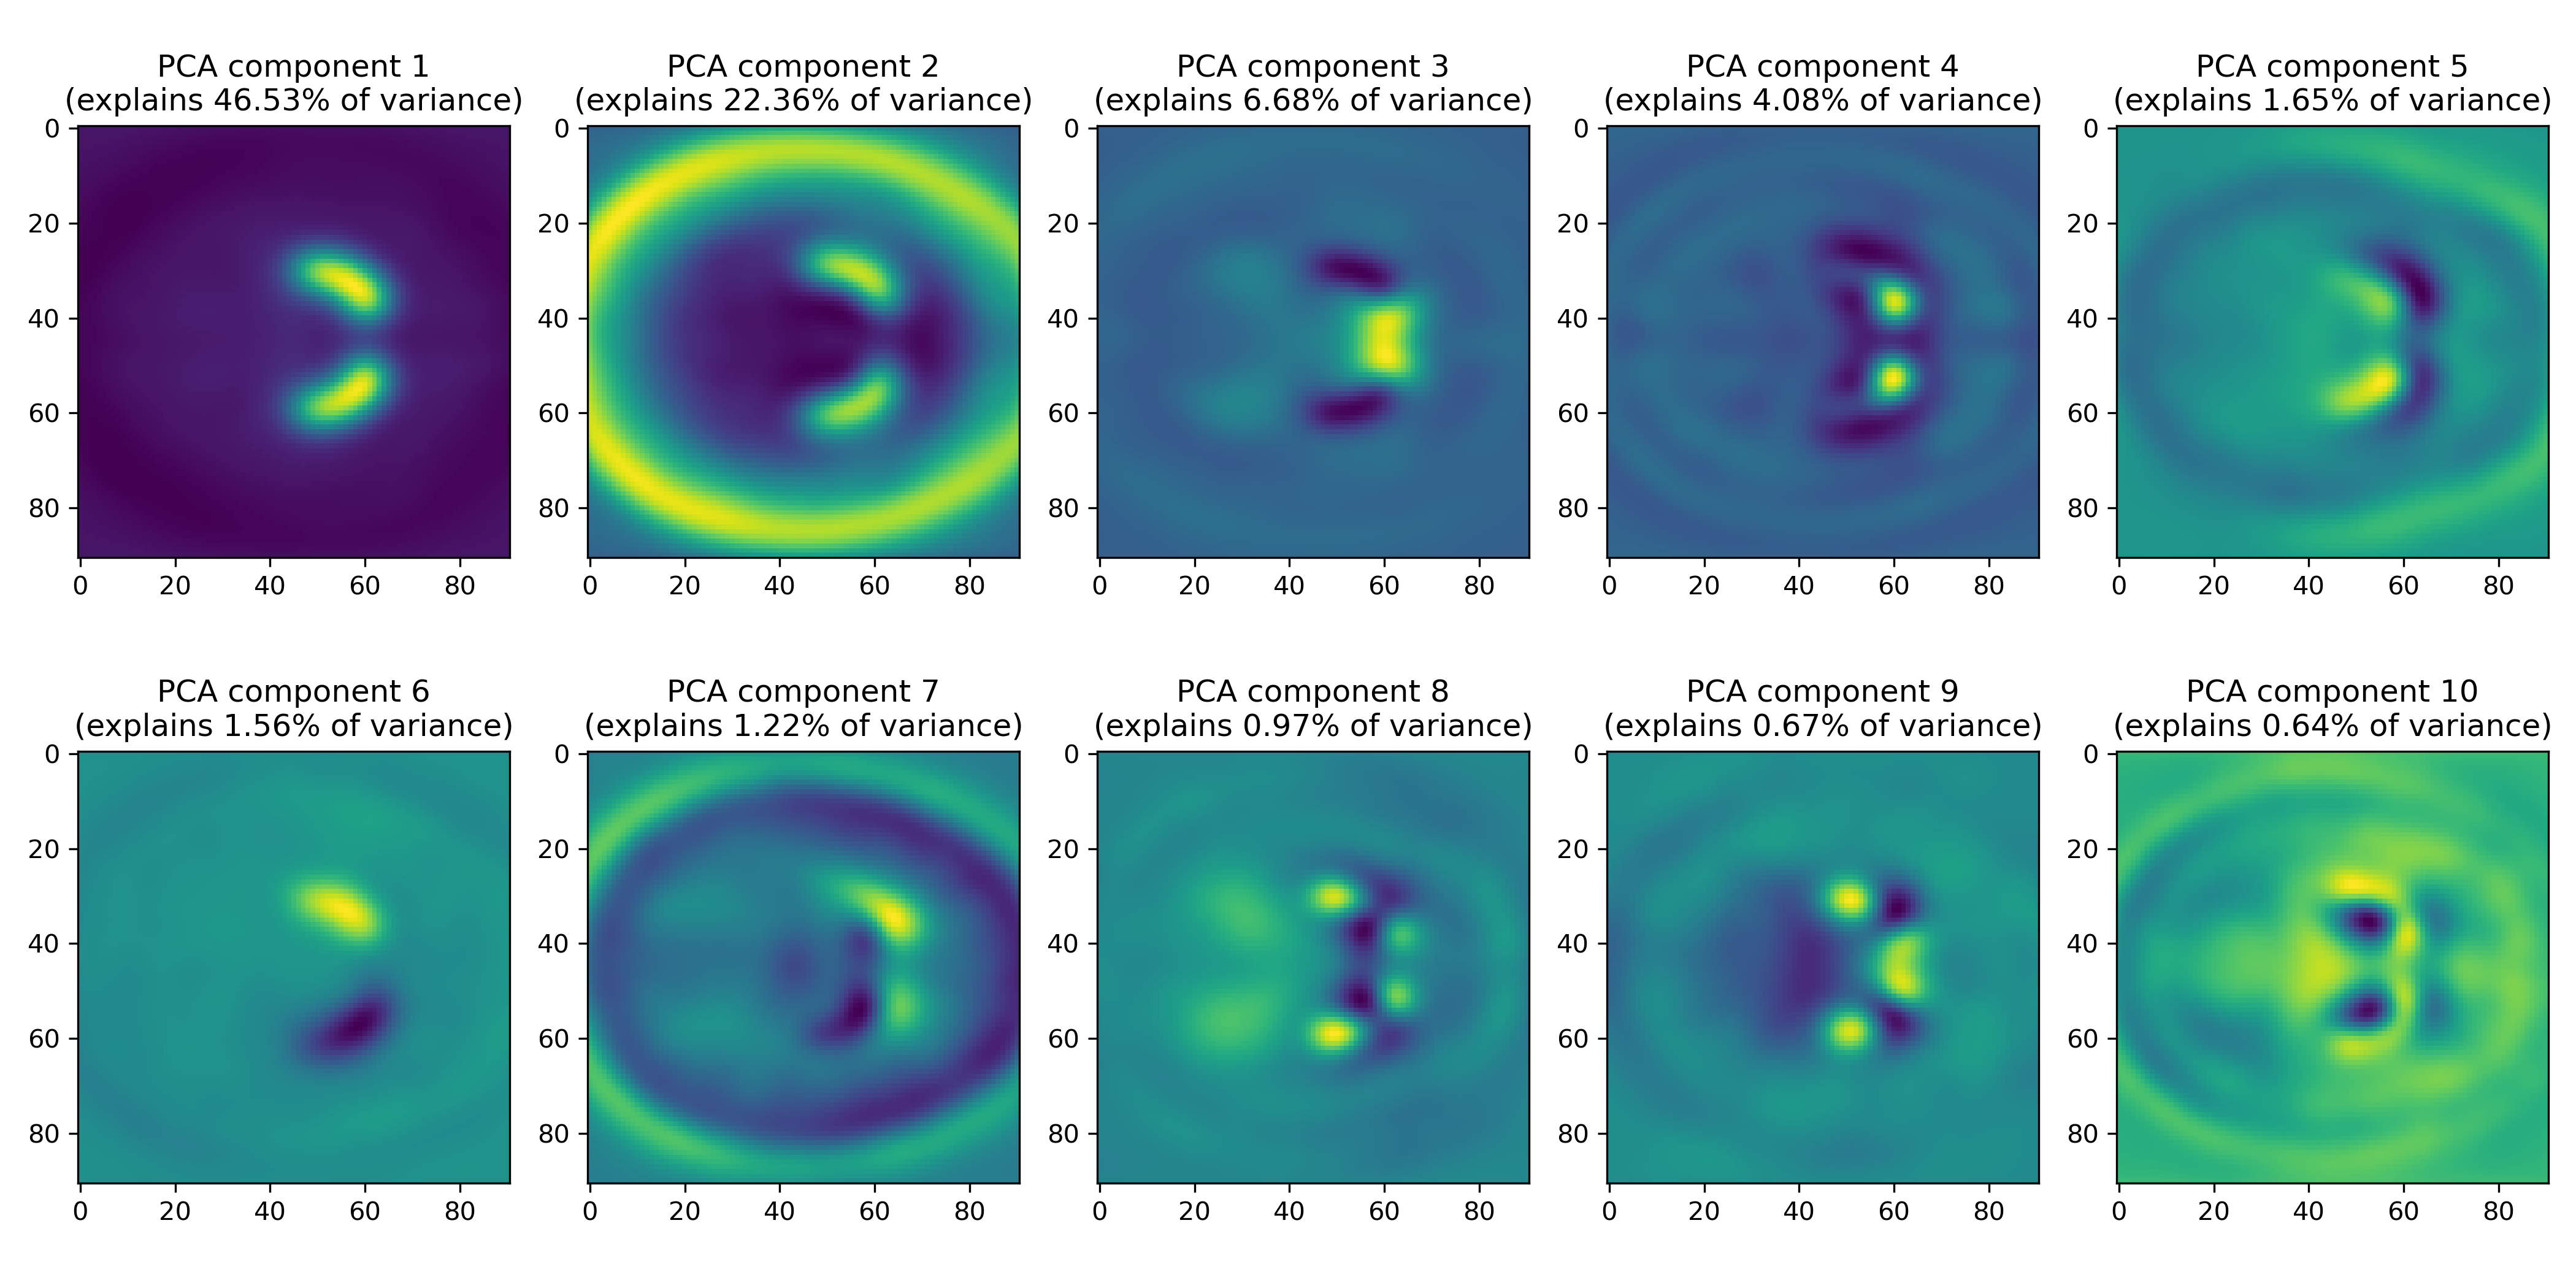
\includegraphics[width=1.0\textwidth]{content/figures/pca_components_splittrain.png}
  \caption{Principle components of the training set (development dataset) for one of the random splits.} 
  \label{fig:pca_components}
\end{figure} 

\subsection{CNN-based classification - MVT and RLT}
\label{subsec:cnn_based_classification_mvt_rlt}



\subsection{CNN-based classification - Regression}
\label{subsec:cnn_based_classification_regression}



\subsection{Determination of Inconclusive Ranges on the Probabilistic Output}
\label{subsec:determinationInconcl}


// TODO

On the validation set...

Determination of inconclusive ranges given a set of target percentages of inconclusive cases (0.2\% to 20.0\%, step 0.2\%).

e.g. what is the inconclusive range corresponding to 10\% of test cases being classified as inconclusive?

The determined inconclusive ranges were then used to compute the balanced accuracy on the conclusive cases.
